\section{The Caking Algorithm}

The purpose of a caked plot is to make a radial 
($r$ vs $\theta$) plot of the data as it would have 
appeared on the imagined untiled detector shown in 
figure~\ref{PhysicalSetup}. By plotting $r$ vs $\theta$,
we will turn circle (of constant $r$ into straight lines 
and we will really distort straight lines.
To create this plot, we will work with the 
convenient quantities $Q$ and $\chi$. Remember that
from equation \ref{qterms2theta} that $Q$ is
related by the sin function to $2\theta$ and that
from equation \ref{2thetatermsr} that $2\theta$
is related to the distance $r$ on the untilted 
detector by the tangent function. 
Consequently, although the relationship is not 
strictly linear, $Q$ will increase as $r$ increases
and therefore $Q$ is an analogous quantity to $r$.
Also, $\chi$ corresponds to the angle radially
around the center of the image. So a cake is really
defined as an intensity plot of the diffraction 
image where the two axis are $Q$ and $\chi$.

To calculate a cake plot, the program implements
the following algorithm. The program has to somehow bin 
$Q$ and $\chi$ space. The code itself can try to pick
a range large enough to encompass all of the 
pixels inside of the diffraction image. Alternately,
the user can specify by hand the exact range that
they want to have caked. But once the bins are
specified, the program has to fill each bin with
intensity values. Since each bin has some 
particular $Q$ and $\chi$ value\footnote{Technically,
each bin has a $Q$ and $\chi$ range, but we will
take the middle of each of these ranges to be the
particular $Q$ and $\chi$ value corresponding to the
bin.} we can calculate the corresponding $(x''',y''')$
pixel coordinate for this bin using~\ref{invertx} and 
\ref{inverty}. We can then
look inside the loaded diffraction data for
this particular intensity value corresponding
to the $(x''',y''')$ value. This intensity then
gets placed inside the bin. $(x''',y''')$
is generally a floating point number so we should
do a bilinear interpolation of the intensity values
to get a best guess.

In principle, the caking algorithm could be implemented
differently. The way it is coded up is to loop over
all the bins. But one could equally well have looped over
all the pixels of diffraction data. Each pixel has a
particular $(x''',y''')$ coordinate. We could use
equations~\ref{ytermsydoubleprime} and
equation~\ref{xtermsxdoubleprime} to calculate the $Q$
and $\chi$ value corresponding to this coordinate. We
could then add the intensity value corresponding to the
$(x''',y''')$ value into the bin which contains the
$Q$ and $\chi$ value. After doing this for all the pixels
in the image, we could then average all the cake bins.
This method would be more accurate because each of the 
pixels in the diffraction image would be used in the analysis
where as they are not necessarily all used above. The major
downside to this implementation is that it does not 
necessarily put an intensity value into all the bins, where 
as the method above does. This code be overcome by applying
the above algorithm at the end only to the bins for which
nothing was put into. But the biggest downside of this 
algorithm is that it is substantially slower because there
are usually significantly more pixels in the diffraction
image then bins used in a cake. For example, mar3450 data
holds $3450\times 3450$ pixels while cakes are typically set
to have a resolution of $600\times 600$. Although
this alternative algorithm was not implemented in the code,
it would in principle be easy to code up and it might
be more desirable in some situations.

Finally, the program can allows for masking of the cake.
Whenever the program finds an intensity value
that should be masked (either because it is too 
large, too small, or in a polygon mask), it fills
in that part of the caked array with a particular 
negative value that describes exactly why the
program was ignored.

Finally, the program can perform a polarization 
correction to the cake. The polarization 
correction formula is
\begin{align}
    I&=Im/PF \\ 
    PF&=P(1 - (\sin(2\theta)\sin(\chi-90))^2) + 
    (1 - P)(1 - (\sin(2\theta)\cos(\chi-90))^2)
\end{align}
with $Im$ the measured intensity. What happens
then is that all pixels have their intensity
value corrected by this formula before they
are put into the caked array. Note that the 
$2\theta$ and $\chi$
values correspond to the particular value
that is being corrected.

\section{Caking with the Program}

\begin{SCfigure}[1][htb]
    \centering
    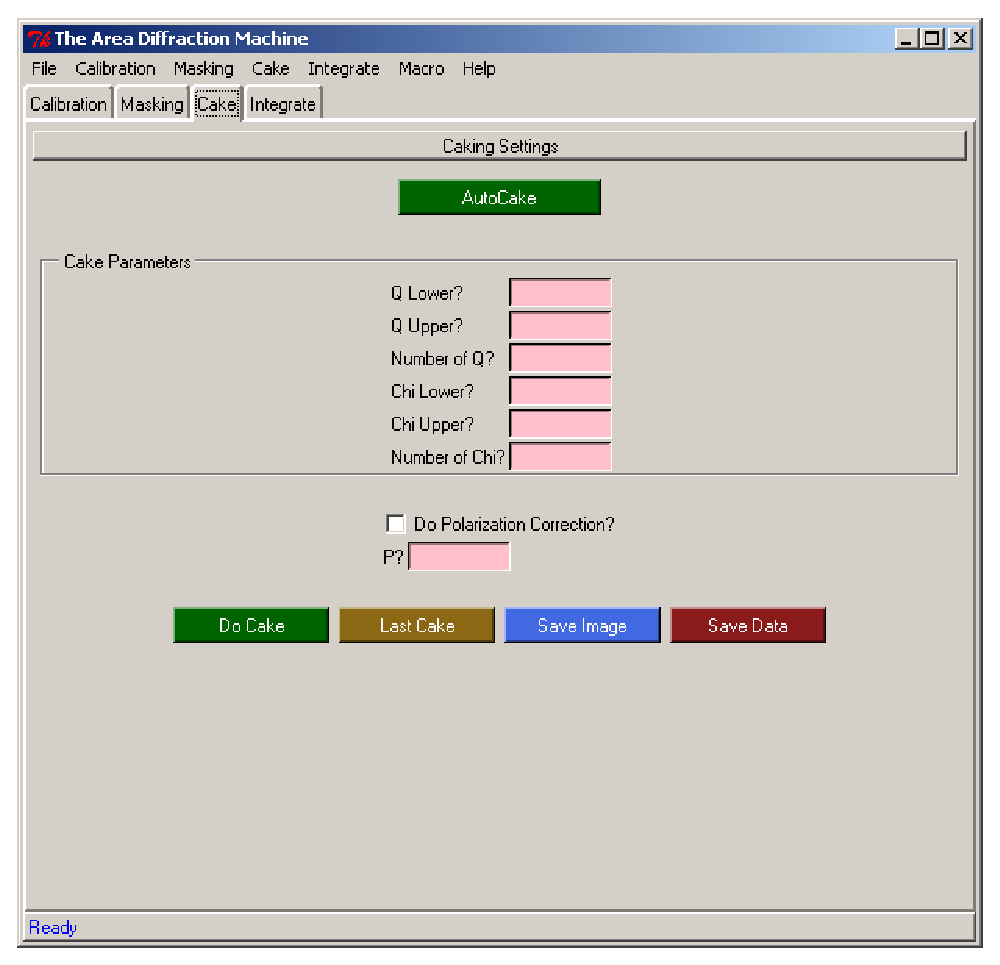
\includegraphics[scale=.75]{figures/caking_tab.eps}
    \caption{A screen shot of the caking tab to 
    the program.  This is the tab where you can 
    cake data.} 
    \label{caking_tab}
\end{SCfigure}

In order to perform a cake with the program, you will have
to already have load into the program one or more
diffraction data files and you will have to input
calibration data into the program. Figure~\ref{caking_tab}
shows the \gui{Caking} tab. This is where caking is done. 
In order to cake the data, the program will need to know a range
in $Q$ and $\chi$ space that should be caked. 
This can be inputted with the \gui{Q Lower?}, \gui{Q Upper?}
\gui{Chi Lower?}, and \gui{Chi Upper?} inputs.
It will also need to know how many $Q$ and $\chi$ bins to 
create when creating the caked data. This can be inputted
with the \gui{Number of Q } and \gui{Number of Chi} inputs.
Once this is done, you can push the \gui{Do Cake} button to 
cake the data. 

\begin{SCfigure}[1][htb]
    \centering
    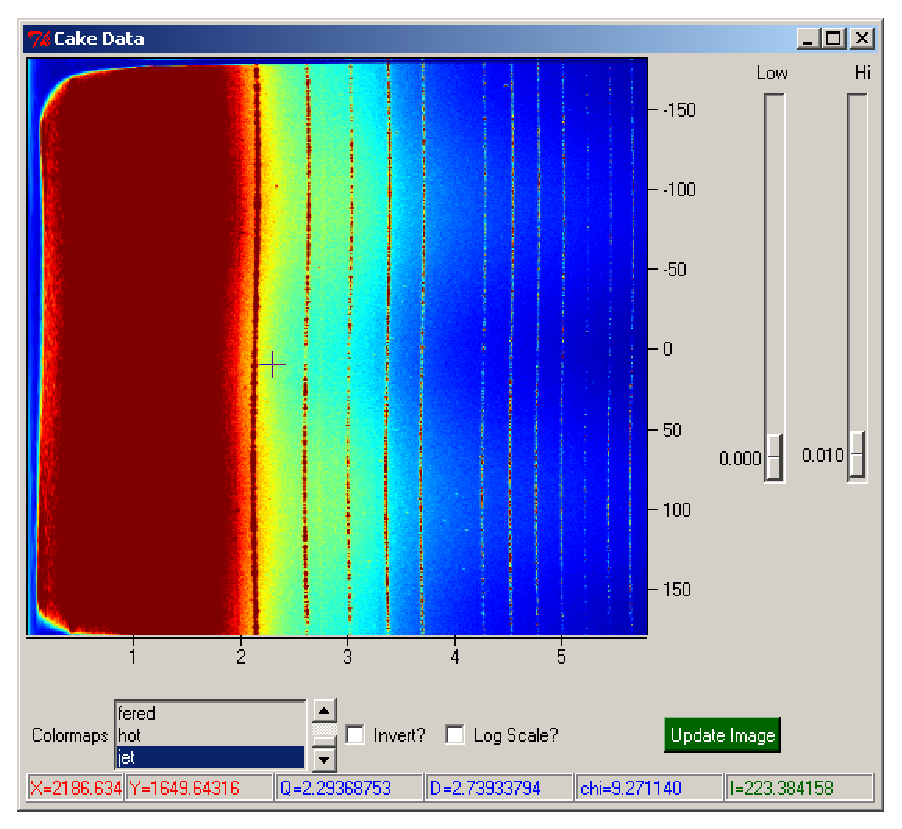
\includegraphics[scale=.75]{figures/cake_data_window.eps}
    \caption{A screen shot of the cake data window for
    the program. This window will open up after the
    data is caked. This window behaves exactly like 
    the diffraction data window.} 
    \label{cake_data_window}
\end{SCfigure}

After the caked data is created, the program will open up a cake data
window which displays the cake data interactively.
The cake data window is just like the diffraction
data window so everything said in Chapter~\ref{viewing_data} 
carries over. The only real difference is that whenever
you zoom into the caked data, the program will take the user
selected zoom range and put it into the range inputs on
the cake tab.

To undo to whatever range was previously used when caking, 
you can use the \gui{Last Cake} button to go back to the
previous cake values. You can do this by 
right clicking on the caked window. (This is just like
zooming out of the diffraction window). 

\section{AutoCake}

The program also has the convenience button \gui{AutoCake}.
\gui{AutoCake} will ``guess'' a good range of $Q$ and $\chi$ 
values, put them into the input, and then push the 
\gui{Do Cake} button for you. This lets you get out a 
cake without much work. What hte program thinks is a
good range is one that will put every pixel from the 
diffraction image into the cake. It will than pick
the bins sizes so that each pixel of the displayed 
cake data will correspond to its own bin. This will ensure
that the cake looks as sharp as the computer can draw it.
After the display is resized, the number of bins will
change correspondingly so that the next time you push
\gui{AutoCake} it will make the cake window look sharp again.

\section{\texorpdfstring{Displaying $Q$ and $\Delta Q$ Lines}
    {Displaying Q and delta Q Lines}}
    \label{cakeQlinesandpeaks}

If a $Q$ list has been loaded into the program, 
constant $Q$ lines or $\Delta Q$ lines can be 
displayed on top of the cake data. Remember that 
$Q$ lines on the caked plot are just straight lines. 
The program will display constant $Q$ lines or 
$\Delta Q$ lines on top of the caked plot whenever they 
should be displayed on the diffraction image. See 
section~\ref{displayconstQlines} and 
section~\ref{displayconstdQlines}.
Figure~\ref{constant_q_lines_on_cake_image} shows constant
$Q$ lines displayed on a caked plot and 
figure~\ref{constant_dq_lines_on_cake_image} shows constant
$\Delta Q$ lines displayed on a caked plot.

\begin{SCfigure}[1][htb]
    \centering
    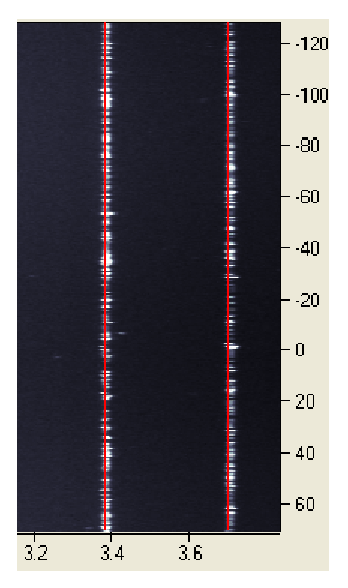
\includegraphics[scale=.75]{figures/constant_q_lines_on_cake_image.eps}
    \caption{A screen shot of the caked data window
    with constant $Q$ lines drawn on top of it.}
    \label{constant_q_lines_on_cake_image}
\end{SCfigure}

\begin{SCfigure}[1][htb]
    \centering
    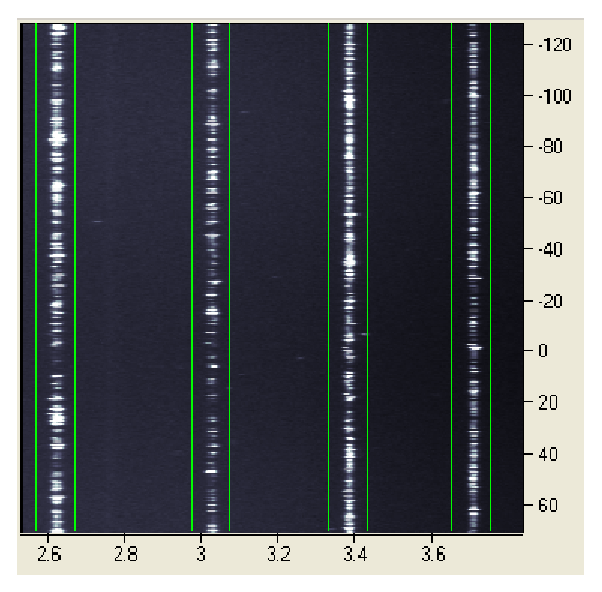
\includegraphics[scale=.75]{figures/constant_dq_lines_on_cake_image.eps}
    \caption{A screen shot of the caked data window
    with constant $\Delta Q$ lines drawn on top of it.}
    \label{constant_dq_lines_on_cake_image}
\end{SCfigure}


\section{Displaying Peaks}\label{displaying_peaks_cake}

\begin{SCfigure}[1][htb]
    \centering
    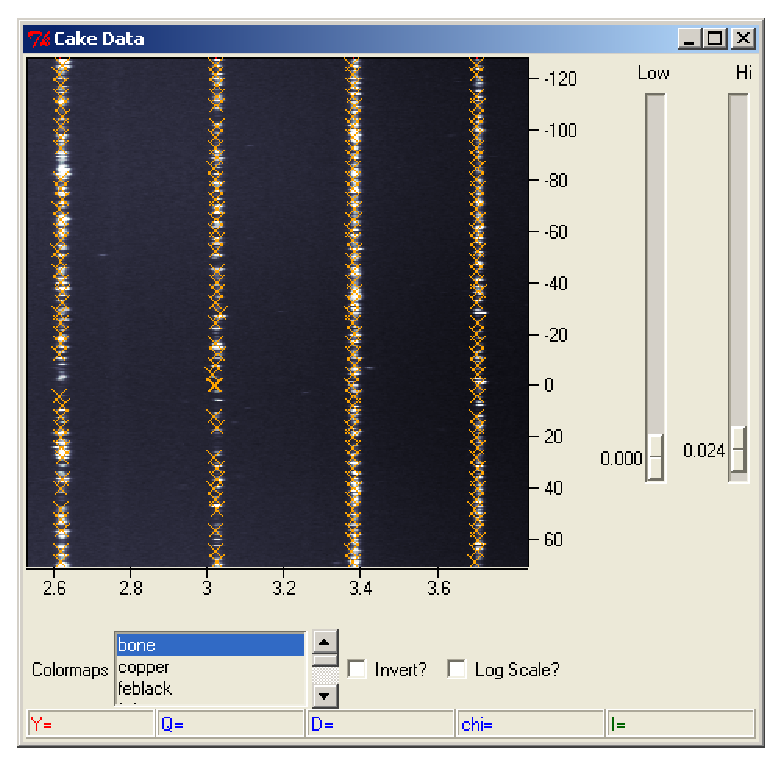
\includegraphics[scale=.75]{figures/peaks_on_cake_image.eps}
    \caption{A screen shot of the caked data window
    with diffraction peaks drawn on top of it.}
    \label{peaks_on_cake_image}
\end{SCfigure}

Any peaks that the program finds when performing
a calibration can be displayed on top of the caked
data. The peaks will be displayed as crosses.
Figure~\ref{peaks_on_cake_image} shows peaks
displayed on a caked plot. Peaks will be displayed on 
the caked plot whenever they should be displayed on 
the diffraction image. See section~\ref{displaying_peaks_diffraction}.

Being able to display $Q$ lines and peaks can
be very useful for checking if a calibration was 
done properly. Figure~\ref{calibration_cake} shows
why this is the case. 

\begin{figure}[htb]
    \centering
    \subfloat[A bad calibration]{
    \label{bad_calibration_cake_zoom_peaks}
    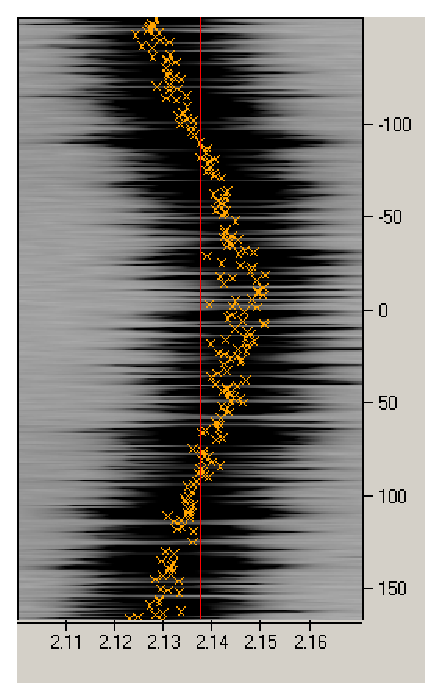
\includegraphics[scale=.75]{figures/bad_calibration_cake_zoom_peaks.eps}}
    \subfloat[A good calibration]{
    \label{good_calibration_cake_zoom_peaks}
    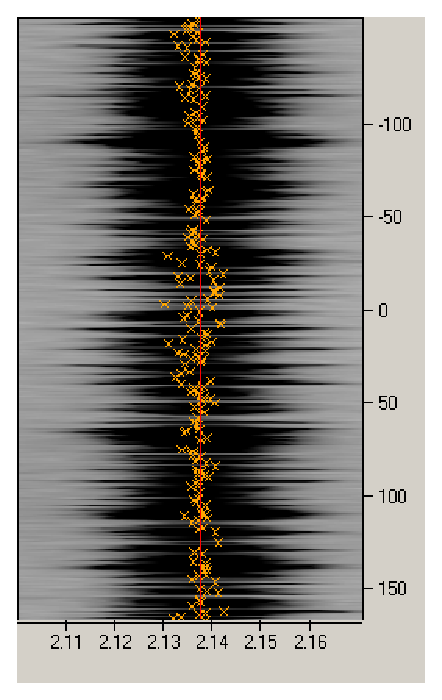
\includegraphics[scale=.75]{figures/good_calibration_cake_zoom_peaks.eps}}		
    \caption{A use of displaying peaks on top of the caked 
    data. Displaying the peaks found while calibrating can 
    be used to help tell if a proper calibration of caked 
    data has been done. Ideally, all the peaks will cluster 
    very close to the $Q$ line and there will be no systematic 
    variation of the peaks around the $Q$ value. If a bad 
    calibration was done, there will be this sort of
    distortion. This can easily be used to test if the
    program is properly calibrating your data.}
    \label{calibration_cake}
\end{figure}


\section{Polarization Correction}
The program can apply a polarization correction to the
cake. To apply a polarization correction, you have
to check the \gui{Do Polarization Correction?} check box
and then input the value into the \gui{P?} input.

\section{\texorpdfstring{Working in $2\theta$}{Working in 2theta}}

You can do everything related to caking in the variable
$2\theta$ instead of $Q$. To do so, you can go into
the file menu and select \gui{Work in 2theta}. When you 
do this, all of the names in the program will switch 
from $Q$ to $2\theta$. You will be asked to input 
$2\theta$ Lower, $2\theta$ Upper, Number of $2\theta$. 
The program will then display the cake image with
$2\theta$ as its axis.

\section{Saving Cake Images}

You can save caked
data out as a \gui{jpg}, \gui{gif}, \gui{eps}, \gui{pdf}, 
\gui{bmp}, \gui{png}, or \gui{tiff}.
When you save out the image as a popular image format, it
will save out the cake image with whatever threshold masks,
polygon masks, $Q$ lines, $\Delta Q$ lines, and peaks that
were displayed over the caked data as it is displayed by
the program.

\section{Saving Cake Data}

You can also save out the caked data in plain text. To do so,
you just have to push the \gui{Save Data} button and
select where to save it. The format of the file is a really
long comment string followed by the data 

\begin{lstlisting}[caption={'The Cake Data Header'}]
# Cake of: N:/data/LaB6_14_02_56.mar3450 
# Data Caked on Wed Mar 12 21:30:55 2008
# Calibration data used to make the cake:
#   x center:    1725.0000000 pixels
#   y center:    1725.0000000 pixels
#   distance:     125.2960000 mm
#   energy:     12735.3957721 eV
#   alpha:          0.0000000 degrees
#   beta:           0.0000000 degrees
#   rotation:       0.0000000 degrees
#   pixel length:     100.0000000 microns
#   pixel height:     100.0000000 microns
# A Polarization correction was applied
#   P = 0.500000
# A greater than mask was applied
#   Greater than mask = 1000.000000
# A Less Than Mask was applied
#   Less than mask = 10.000000
# Polygon mask(s) were applied
# Polygon(s) used in the analysis:
#   2400.10912343	1073.5706619
#   962.511627907	2282.88014311
#   2850.51520572	2572.86762075
#
#   1573.33631485	1215.47942755
#   1820.13416816	2893.70483005
#   2906.04472272	1573.33631485
# Cake range:
#   Q Lower = 0.000000
#   Q Upper = 6.726544
#   Number of Q = 560.000000
#   Q Step = 0.012012
#   chi Lower = -180.000000
#   chi Upper = 180.000000
#   Number of Chi = 560.000000
#   chi Step = 0.642857
# Note: pixels outside the diffraction image are saved as -1
#   Pixels greater than the greater than mask are saved as -2
#   Pixels less than the less than mask are saved as -3
#   Pixels inside of a polygon masks are saved as -4
# chi increased down. Q increases to the right
\end{lstlisting}
As you can see, the comment string is supposed to be as verbose
and useful as possible. The idea was to put into it as much
information about possible about under exactly what conditions
the cake was done. The first thing in the comment string is
the name of the file that was caked. If multiple files were loaded
and the sum image was caked, all of the files will be put into
the comment string. Next is a printout of the calibration values
used while caking the data. Next is the polarization correction,
greater than mask and less than mask that were used. It will print
out the pixel coordinates of any polygons that were applied to
the cake image. It prints out the cake range that is used.

Finally, the program codes special bins in the output caked data
with special values. Any bins that are outside of the diffraction
image in cake space are saved as -1. Any bins that were masked
because they were too large are saved as -2. Any bins that
were masked because they were too small are saved as -3. Any bins 
that were inside of a pixel mask are saved as -4. This is all
displayed in the comment string. The program tries to be smart about
the comment string. If no polygon masks were used, the comment string
instead contains lines like
\begin{lstlisting}[caption={'Alternate Header'}]
# No polarization correction was applied
# No greater than mask was applied
# No less than mask was applied
# No polygon masks were applied
\end{lstlisting}
If the program is working in $2\theta$ mode, the inputs will instead 
say \gui{2theta Lower}, etc. The comment string will instead have
\begin{lstlisting}[caption={'Another Alternate Header'}]
#   2theta Lower = 0.000000
#   2theta Upper = 62.814525
#   number of 2theta = 560.000000
#   2theta Step = 0.112169
\end{lstlisting}
Following the comment string is the data. The format for the data is
that each line corresponds to a different $\chi$ bin and each of the 
values for a particular $Q$ bins is separated by a space. Just
as the comment string explains, chi increased down and Q increases to 
the right. 

